\documentclass[12pt]{article}

\usepackage[margin = 30mm]{geometry}
\usepackage{abstract}
\usepackage{titlesec}
\usepackage{titletoc}
\usepackage{tikz}
\usetikzlibrary{trees}
\usepackage{fancyvrb}
\usepackage{xcolor}
\usepackage{amssymb}



\setlength\parindent{0pt}
\frenchspacing

\usepackage{hyperref}
\hypersetup{
    colorlinks,
    linktoc = all,
    citecolor=black,
    filecolor=black,
    linkcolor=black,
    urlcolor=black
}

\titleformat{\section}{\center\bf \large}{\thesection.}{0.5em}{}
\titleformat{\subsection}{\center\bf}{\thesubsection.}{0.5em}{}



\newcommand{\localtextbulletone}{\textcolor{black}{\raisebox{.35ex}{\footnotesize$\bullet$}}}
\renewcommand{\labelitemi}{\localtextbulletone}



\titlecontents{section}
	[0pt]
	{ }
	{\contentsmargin{0pt}\thecontentslabel.\enspace\normalsize}
	{\contentsmargin{0pt}\normalsize\MakeUppercase}
	{\titlerule*[.5pc]{}\contentspage}
	[]

\titlecontents{subsection}
	[15pt]
	{ }
	{\contentsmargin{0pt}\thecontentslabel\enspace\normalsize}
	{\contentsmargin{0pt}\normalsize\MakeUppercase}
	{\titlerule*[.5pc]{}\contentspage}
	[]





\setcounter{tocdepth}{1}

\title{Standardisation Guide for ``\texttt{rbf-tools}''}
\author{N.K. - \texttt{kraemer@ins.uni-bonn.de}}
\begin{document}
\maketitle
\begin{abstract}
The purpose of this guide is to collect any standardisation I have come up with over time. On top of that, I mention other guidelines, like naming conventions, structure conventions and more. 
\end{abstract}
\begin{figure}[h]
\centering
\begin{minipage}{0.5\textwidth}
\tableofcontents
\end{minipage}
\end{figure}




\section{Purpose of the module}

The purpose of the module is to collect most of the things I have programmed in the past 18 months with regard to radial basis functions. This collection is supposed to be handed over, eventually, without losing any reusability possibilities--i.e. I should not be the only one who understands this.\\

Resuability is a driving force of most of the modules. Many features have to be used in almost every script; for instance, building a kernel matrix. I got sick of doing it from scratch everytime, hence I started this collection.


\section{Hierarchy}
The hierarchy is supposed to be as flat as possible. The only things that are supposed to be in directories are figures and pointsets; see Figure \ref{fig:hierarchy}.

\begin{figure}[h]
\centering
\tikzstyle{every node}=[draw=black,thick,anchor=west]
\tikzstyle{selected}=[draw=red,fill=red!30]
\tikzstyle{optional}=[dashed,fill=gray!50]
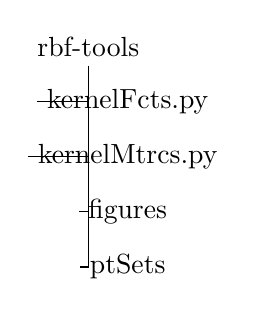
\begin{tikzpicture}[%
	grow via three points={one child at (0.5,-0.7) and
 	two children at (0.5,-0.7) and (0.5,-1.4)},
	edge from parent path={(\tikzparentnode.south) |- (\tikzchildnode.west)}]
	\node {rbf-tools}
    		child { node {kernelFcts.py}}		
    		child { node {kernelMtrcs.py}}
    		child { node {figures}}
   		child { node {ptSets}};
\end{tikzpicture}
\caption{File structure of \texttt{rbf-tools}}
\label{fig:hierarchy}
\end{figure}


\section{Naming and coding conventions}
I follow naming conventions with two purposes in mind:
\begin{enumerate}
\item Good programming practice
\item Unification
\end{enumerate}

\subsection{Good naming practice}
The following is a list of most naming conventions regarding good practices:
\begin{enumerate}
\item \textbf{Variable naming:} 
\begin{itemize}
\item \textbf{Descriptive naming:} do not use \texttt{x}, \texttt{N} or \texttt{K}, but \texttt{pt}, \texttt{numPts} or \texttt{kernelMtrx}
\item \textbf{Short names:} do not use \texttt{standardKernelMatrixWithMaternKernel}, but \texttt{kernelMtrx}
\item No underscores (privilege of python)
\item No all-uppercase variables (privilege of python)
\item Indicate new ``term'' with a single uppercase letter: \texttt{kernelFct}, \texttt{kernelMtrx}, \texttt{ptSet}
\end{itemize}
\item \textbf{Commenting:} As long as the variables are named well, I do not need comments except for very few occasions
\item \textbf{Function naming:} verb-noun scheme, i.e. \texttt{buildKernelMtrx}, \texttt{getPtSet}, ...
\item \textbf{File naming:} Each file has to include the following information:
\begin{enumerate}
\item \textbf{Name:} e.g. \texttt{'interpolation.py'}
\item \textbf{Purpose:} Describe the purpose of the file in a single sentence (if that is not possible, think again about starting this file at all)
\item \textbf{Description:} Describe the method in two or three sentences giving the main keywords
\item \textbf{Author:} Usually me
\end{enumerate}
An exemplary header is the following, taken from \texttt{'interpolMatern1d.py'}:
\begin{Verbatim}[formatcom=\color{blue!50!black}]
# NAME: 'interpolMatern1d.py'
#
# PURPOSE: Basic 1-dimensional interpolation using Matern functions
#
# DESCRIPTION: I solve a system involving a Matern-kernel matrix 
# where the Matern kernel is based on scipy.special's functions
# and plot the 10-th Lagrange function.
#
# AUTHOR: NK, kraemer(at)ins.uni-bonn.de
\end{Verbatim}
\end{enumerate}

\subsection{Unification}
The following is a list of most naming conventions regarding a unified system:
\begin{enumerate}
\item \textbf{Kernel functions:} I refer to kernel functions and kernel matrices using \texttt{kernel}, not \texttt{kern} nor \texttt{cov}
\item \textbf{Common Abbreviations:} I use as common abbreviations:
\begin{itemize}
\item Indices: \texttt{idx}, \texttt{jdx}, \texttt{kdx}, ...
\item Point: \texttt{pt}
\item Pointset: \texttt{ptSet}
\item Numer of points: \texttt{numPts}
\item Matrix: \texttt{mtrx}, matrices: \texttt{mtrcs}
\item Length of a vector called \texttt{vecAbc}: \texttt{lenVecAbc}
\item Pointset for evaluation (plotting): \texttt{evalPtSet}
\item Number of evaluation points: \texttt{numEvalPts}
\item Lebesgue constant: \texttt{lebCnst}
\item Gaussian: \texttt{gauss} (as in \texttt{gaussKernel} instead of \texttt{gaussianKernel})
\end{itemize}
\end{enumerate}




\subsection{Other good practices}
\begin{enumerate}
\item \textbf{Functions:}
\begin{itemize}
\item Each function should serve \textbf{a single} purpose which should be clear from the naming
\item Each function should be deterministic, i.e. two runs with the same input give the same output; see next point
\end{itemize}
\item \textbf{Seeds for random numbers:} Each file should always give the same result as long as nothing is changed. Hence, start everything that includes random numbers with \texttt{np.random.seed(15051994)}
\item Readability of a program often trumps performance
\end{enumerate}

\section{Files}

In the following I describe some files and their standardisations.



\subsection{Kernel functions}
	\label{sec:kernelFct}
I collect kernel functions in the file \texttt{kernelFcts.py}. They all take two points as inputs and give out a scalar. As an example, the Gaussian:
\begin{Verbatim}[formatcom=\color{blue!50!black}]
def gaussKernel(x,y, lengthScale = 1.0):
    return np.exp(-np.linalg.norm(x-y)**2/(2*lengthScale**2))
\end{Verbatim}

The distance of the two inputs, $x$ and $y$, is computed inside the function. The purpose of this is that I can construct kernel matrices in a very easy manner. 

\subsection{Kernel matrices}
I collect kernel matrices in the file \texttt{kernelMtrcs.py}. The all take two pointsets as inputs and return a matrix. As an example, the standard kernel matrix: 
\begin{Verbatim}[formatcom=\color{blue!50!black}]
def getKernelMtrx(ptSetOne, ptSetTwo, kernelFct):
    lenPtSetOne = len(ptSetOne)
    lenPtSetTwo = len(ptSetTwo)
    kernelMtrx = np.zeros((lenPtSetOne, lenPtSetTwo))
    for idx in range(lenPtSetOne):
        for jdx in range(lenPtSetOne):
            kernelMtrx[idx,jdx] = kernelFct(ptSetOne[idx,:], ptSetTwo[jdx,:])
    return kernelMtrx
\end{Verbatim}

The input pointsets need to have the same dimension, but do not need to match in size. The kernel function \texttt{kernelFct} needs to be of the form I described in section \ref{sec:kernelFct}

\end{document}